\section{Model Predictive Control and Learning}	\label{sec: MPC_3}
We present a Model predictive control (MPC) scheme that uses Gaussian process transition models and is capable of online learning. To this end, we employ the GP model and GP Transition model for long-term prediction. we formulate the considered control problem and present the online learning scheme of the Gaussian process model predictive control and we denote it as GP-MPC. 


The chapter starts with an introduction (Section \ref{sec:section3.1}) to the topic of Model Predictive Control and its challenges, along with the mathematical basics of MPC, together with a detailed discussion of feasibility and stability required later for the main theoretical results of this chapter. In \ref{sec:section3.2}, we formulate the considered control problem and present the online learning scheme of GP-MPC and also the resulting optimal control problem. 


\subsection{Model Predicitve control}\label{sec:section3.1}
Model Predictive Control (MPC, \cite{rawlings2009model}) is a control methodology adept at managing multi-input multi-output systems, accommodating constraints from the outset of the design process. Essentially, MPC operates as iterative optimal control, leveraging a model of a real process $x_{k+1} = f(x_k,u_k)$, with state $x_k$ and input $u_k$ at time $k$, for prediction and to address a finite horizon optimal control problem (OCP). The initial computed optimal input sequence is applied to the plant, and the OCP is resolved at the subsequent time step. This approach considers potential disturbances and uncertainties occurring between consecutive time steps. The recurrent solving of the OCP at each time instant advances the prediction horizon by one step, hence the term receding horizon control\cite{mayne2000constrained}.

In terms of performance, Model Predictive Control often outperforms other control methods due to its ability to predict future process behavior, enabling the computation of control actions based on anticipated outcomes. Additionally, MPC allows for the incorporation of preview information about references and disturbances, if available. Unlike many other control approaches, MPC facilitates the direct consideration of constraints on input, state, and output during the design phase. This feature has garnered significant scientific interest and found practical applications. Over the past decades, a robust theoretical framework has been developed to provide guarantees concerning aspects like recursive constraint satisfaction and stability.

However, despite the advantages it offers, MPC also presents challenges. For example, the standard MPC formulation necessitates full state information, meaning the entire state $x_k$ must be measurable. If this requirement cannot be met, various state estimation methods, such as Luenberger observers, Kalman filters, or more sophisticated techniques like moving horizon estimation \cite{rawlings2006particle}, can be employed. Alternatively, output feedback MPC schemes that solely utilize measured system output offer an alternative approach.

Another challenge is the potentially high computational costs associated with MPC. Solving the (possibly nonlinear and nonconvex) optimal control problem within the sampling time frame is crucial. Initially, this constraint limited MPC deployment to systems with large time constants, such as process industry plants. However, advancements in algorithms, such as acados \cite{verschueren2019acados}, and the increasing computational power of digital processors now permit the use of MPC in more demanding applications, including embedded systems for mechatronics \cite{zometa2012implementation}. Moreover, MPC's scope extends beyond traditional engineering tasks, with applications in diverse fields such as HIV treatment strategies in medicine \cite{hernandez2014switching} and others \cite{mayne2014model}. The basic procedure applied by a model predictive control scheme can be illustrated in Figure \ref{f:figure_mpc} and summarized as follows:

\begin{enumerate}
    \item Obtain the state $x_k$ at the current time step $k$.
    \item Formulate and solve a finite horizon optimal control problem. This involves predicting the future evolution of the system and determining an optimal input sequence that minimizes a given cost function over a finite prediction horizon.
    \item Apply the first part of the optimal input sequence to the system. 
    \item Repeat, go back to Step 1.
\end{enumerate}

 \begin{figure}[ht]		% h - here, t - top, b - bottom, p - page, ! - try hard
  \centering
  \afig{1.3}{figures/mpc}			% {scaling}{Figure from MATLAB, picture, etc.}
  \caption{MPC Illustration: For a particular initial condition $x_k$ at time instant $k$, a predicted open-loop sequence of inputs $\hat{u}$ is computed up to a prediction horizon $N$. The input sequence, together with the resulting predicted states $\hat{x}$, are computed in such a way that they minimize a given cost\cite{maiworm2021gaussian}.}
  \label{f:figure_mpc}
\end{figure}

\subsubsection{MPC formulation} \label{sec:Section 3.2}
We consider discrete-time-invariant and constrained nonlinear state-space systems of the form:
\begin{equation}\label{eq:dt_nl_dynamics}
\begin{aligned}
 x_{k+1} & = f(x_k,u_k) \\
 & u_k \in \mathcal{U} \\
& x_k \in \mathcal{X}
\end{aligned}
\end{equation}

where \( k \in \mathbb{N}_0 \) denotes the discrete time, \( x_k \in \mathbb{R}^{n_x} \) represents the state, and \( u_k \in \mathbb{R}^{n_u} \) denotes the input. 

The state and input constrained sets are subsets of the respective spaces, i.e., \( X \subset \mathbb{R}^{n_x} \) and \( U \subset \mathbb{R}^{n_u} \). Input constraints usually arise due to actuator saturation, for example, a valve cannot be opened more than 100\% and not less than 0\%. State constraints often arise as a consequence of process operation conditions, for example, if for safety reasons a temperature should not exceed a predefined limit.

A particular initial condition \( x_k \) at time instant \( k \) and a sequence of inputs \( u_k = \{u_k,u_{k+1},\ldots\} \) applied to Equation (\ref{eq:dt_nl_dynamics}) result in a state sequence \( x_k = \{x_k,x_{k+1},\ldots\} \). The state sequence as a whole depends on the initial condition and the applied input sequence, i.e., \( x_k = x_k(x_k,u_k) \). However, for the sake of simpler notation, we do not emphasize this dependence.

For the standard MPC formulation, together with its theoretical results as presented in the following, the common objective is regulation to and stabilization of the origin. Thus, it is assumed that the system possesses an equilibrium point at the origin, i.e., \( f(0,0) = 0 \).

\subsubsection{Prediction Model} \label{sec:prediction model}
In order to compute the future behavior of the process Equation (\ref{eq:dt_nl_dynamics}), a prediction model
\begin{equation}\label{eq:pd_model}
 \hat{x}_{k+i+1|k} = \hat{f}(\hat{x}_{k+i|k}, \hat{u}_{k+i|k})
\end{equation}
is used, which is evaluated over a finite prediction horizon $N \in \mathbb{N}$ where $i \in \{0,1,...,N-1\}$. The variable $k$ denotes the global discrete time, whereas $i$ denotes the internal controller time within the prediction horizon $N$. The hat notation $\hat{(\cdot)}$ denotes a predicted variable and the subset notation $(\cdot|k)$ emphasizes that the prediction is based on the information available at the specific time step $k$. The current measurement $x_k = \hat{x}_{k|k}$ serves as the initial condition for the prediction. The Long-term prediction model is explained in detail in Section \ref{sec:section2.3}. This GP transition model serves as a prediction model in our case.

Given a predicted input sequence $\hat{u}_{k|k} = \{\hat{u}_{k|k}, \hat{u}_{k+1|k}, ..., \hat{u}_{k+N-1|k}\}$ and initial condition $x_k$, the predicted state evolution is $\hat{x}_{k|k} = \{\hat{x}_{k|k}, \hat{x}_{k+1|k}, ..., \hat{x}_{k+N|k}\}$ with $\hat{x}_{k|k} = x_k$. Note that $\hat{x}_{k|k}$ has $N + 1$ elements, whereas $\hat{u}_{k|k}$ has $N$ elements because no further input is needed in the last stage. The difference between the signal sequences $u_k$ and $x_k$ of the real process Equation (\ref{eq:dt_nl_dynamics}) and the sequences $\hat{u}_{k|k}$ and $\hat{x}_{k|k}$ of the prediction model Equation (\ref{eq:pd_model}) is that the predicted sequences are computed for each time instant $k$ and used as internal variables of the controller, whereas $u_k$ and $x_k$ describe the applied control inputs and actual system evolution over time.

\subsubsection{Cost Function} \label{sec:costfunc}
The model predictive controller operates by computing an open-loop input sequence $\hat{u}_{k|k}$ through the minimization of a cost function over a finite horizon $N$ starting from the initial condition $x_k$. 

\begin{equation}\label{eq:cost_function}
    V_N(x_k,\hat{u}_{k|k}) = \sum_{i=0}^{N-1} \ell(\hat{x}_{k+i|k}, \hat{u}_{k+i|k}) + V_f(\hat{x}_{k+N|k})
\end{equation}

This cost function, denoted as $V_N(x_k,\hat{u}_{k|k})$, is comprised of a stage cost $\ell(x,u)$ and a terminal cost $V_f(x)$, as shown in Equation (\ref{eq:cost_function}).

The stage cost penalizes deviations of the predicted state and input trajectories from the origin/set point at each prediction step, while the terminal cost emphasizes penalizing the deviation of the last predicted state. To ensure the stability of the system, Assumption \ref{assumption:assumption1} needs to be met.


\begin{assumption} \label{assumption:assumption1}
    referred to as the Positive Definite Cost assumption, states that both the stage and terminal costs are positive definite and evaluated to zero at the origin:
\begin{itemize}
    \item $\ell(0,0) = 0$ and $\ell(x,u) > 0$ for all $(x,u) \neq (0,0)$.
    \item $V_f(0) = 0$ and $V_f(x) > 0$ for all $x \neq 0$.
\end{itemize}
\end{assumption} 


It's important to note that the cost function Equation (\ref{eq:cost_function}) does not explicitly rely on the state sequence $\hat{x}_{k|k}$, as it is determined by the given initial condition $x_k$ and the input sequence $\hat{u}_{k|k}$.

A typical control objective involves driving the state to the origin rapidly while ensuring that control energy remains within specified limits. This presents a trade-off that must be considered when selecting a stage cost. Hence, determining the most suitable cost function according to the specific control objective is a significant task on its own.

The common stage cost function used is the quadratic cost function, where the function contains quadratic states and inputs. 
\begin{equation}\label{eq:quadratic cost function}
   \ell(\hat{x}_{k+i|k}, \hat{u}_{k+i|k}) =  \hat{x}_{k+i|k}^T Q \hat{x}_{k+i|k} + \hat{u}_{k+i|k}^T R \hat{u}_{k+i|k}
\end{equation}
where Q and R are matrices chosen to be positive definite, with all off-diagonal elements set to zero. Intuitively, the diagonal elements of Q represent the weighting assigned to individual error signals, while the elements of R represent the weighting assigned to each control action. In practice, as the controller designer, we manually select Q and R based on the desired performance of the system.

\subsubsection{Optimal Control Problem } \label{sec:ocp}
At each time step $k$, the model predictive controller  minimizes the cost function Equation (\ref{eq:cost_function}) concerning the open-loop input sequence $\hat{u}_{k|k}$, while adhering to state and input constraints and maintaining the modeled system dynamics Equation (\ref{eq:pd_model}) and the initial condition $x_k$. Moreover, it ensures that the last predicted state $\hat{x}_{k+N|k}$ lies within a designated terminal region $X_f \subseteq X$, crucial for establishing recursive feasibility (refer to Section feasibility section).

The resulting optimal control problem used in model predictive control is


\begin{equation}\label{eq:ocp_general}
\begin{aligned}
    {P}_N(x_k) : \min_{\hat{u}_{k|k}}\quad & V_N(x_k,\hat{u}_{k|k}) \\
\text{subject to} \quad & \forall i \in I_{0:N-1} : \\
& \hat{x}_{k+i+1|k} = \hat{f}(\hat{x}_{k+i|k}, \hat{u}_{k+i|k}) \\
& \hat{x}_{k|k} = x_k \\
& \hat{u}_{k+i|k} \in \mathcal{U} \\
& \hat{x}_{k+i|k} \in \mathcal{X} \\
& \hat{x}_{k+N|k} \in \mathcal{X_f}
\end{aligned}
\end{equation}

The solution to $P_N(x_k)$ is denoted as $\hat{u}^*_{k|k} = \{\hat{u}^*_{k|k}, \hat{u}^*_{k+1|k}, ..., \hat{u}^*_{k+N-1|k}\}$, where the superscript $*$ signifies the optimal solution. Correspondingly, the resulting optimal state sequence is represented as $\hat{x}^*_{k|k} = \{\hat{x}^*_{k|k}, \hat{x}^*_{k+1|k}, ..., \hat{x}^*_{k+N|k}\}$. The optimal cost is $V^*_N(x_k) = V_N(x_k, \hat{u}^*_k|k)$, typically referred to as the value function. The initial element of the optimal input sequence $\hat{u}^*_{k|k}$, is implemented in the process, thereby defining the MPC control law $u_k = \kappa_{MPC}(x_k) = \hat{u}^*_k|k$. Subsequently, the successor state is updated as $x_{k+1} = f(x_k, \kappa_{MPC}(x_k))$, and the process repeats at the next time step by solving $P_N(x_k)$ again.

As widely recognized, the recursive solution to an optimal control problem doesn't inherently ensure stability. There's no guarantee of feasibility, meaning a solution to the optimal control problem may not exist at the subsequent time instant. However, a robust theory has been developed to ensure feasibility and stability, often employing concepts from Lyapunov stability and set theory, particularly for guaranteeing recursive feasibility. Subsequent subsections delve into these fundamental concepts and methodologies. Only the concept of feasibility is explained in detail while an assumption is made about stability. 

\subsubsection{Feasibility}
Feasibility in the context of model predictive control  encompasses the notions of initial and recursive feasibility. Initial feasibility pertains to the existence of a solution to the initial optimal control problem at $k = 0$, while recursive feasibility ensures that if a solution exists at $k = 0$, it remains attainable at all subsequent time steps $k > 0$.

We commence our exploration with the concept of initial feasibility, where we introduce the notion of admissible inputs, leading to the crucial concept of the feasible set. Additionally, we introduce two fundamental assumptions pivotal for establishing recursive feasibility and later, stability. Subsequently, we delve into recursive feasibility, incorporating further assumptions.

In the subsequent discussion, we consider the nominal scenario where the prediction model aligns with the real process, i.e., there is no error between the prediction model $\hat{f}(x,u)$ and the plant $f(x,u)$. For ease of narrative, we omit the estimation notation $\hat{(\cdot)}$ and the temporal dependency $(\cdot|k)$ throughout this section. Given the focus on the feasibility of optimal control problems, the differentiation between real and predicted variables becomes unnecessary. We occasionally employ $x^+ = f(x,u)$ as shorthand for $x_{k+1} = f(x_k,u_k)$. Much of the content presented here is informed by \cite{limon2006stability,limon2009input,rawlings2009model}.

\textbf{Initial Feasibility :}

Initial feasibility in an MPC scheme pertains to whether the initial optimal control problem yields a solution. In static optimization, a problem of the form,

\[
\text{minimize}\underset{u\in U} J(u)
\]

admits a solution according to Weierstrass's theorem if $J$ is continuous, and $\mathcal{U}$ is a compact and nonempty set \cite{rawlings2009model},\cite{luenberger1969optimization}. Here, $\mathcal{U}$ constitutes the feasible set.

In optimal control problems akin to $P_N(x_k)$, besides the constrained set $\mathcal{U}$, additional constraints arise in the form of a dynamical system $x^+ = f(x,u)$, along with constrained sets $\mathcal{X}$ and $\mathcal{X_f}$. The objective is to ascertain a sequence of control inputs that guides the initial state $x_k$ within a finite prediction horizon to the terminal region $\mathcal{X_f}$ (and ultimately to the origin) at minimal cost while adhering to state and input constraints. Such an input sequence is termed admissible input(feasible input).

\begin{definition}\label{de:definition3.1}
(Admissible input) An input sequence $u = \{u_0,u_1,...,u_{N-1}\}$ is admissible if, for the initial condition $x_0$, the resulting state sequence $x = \{x_0,x_1,...,x_N\}$, and for all $i \in [0:N-1]$, the conditions:
(i) $u_i \in \mathcal{U}$
(ii) $x_i \in \mathcal{X}$
(iii) $x_N \in \mathcal{X_f}$
hold, indicating satisfaction with input constraints and adherence to state and terminal constraints \cite{maiworm2021gaussian}.
\end{definition}

It's worth noting that due to $\mathcal{X_f} \subseteq \mathcal{X}$, $x_N \in \mathcal{X}$. Moreover, an admissible input need not necessarily minimize the cost function; it merely represents a candidate solution for the optimal control problem $P_N(x_k)$.

Admissibility of an input sequence is contingent upon a specific initial state $x_0$, with some initial states admitting admissible inputs while others do not. This distinction is particularly pertinent in MPC, where the initial value often represents the sole variable changing between the current and subsequent optimal control problems. This motivates the introduction of the feasible set.

\begin{definition}\label{de:definition3.2}
   ( Feasible set) The feasible set, denoted as $\mathcal{X_N}$, encompasses all initial states $x_0$ for which at least one admissible input sequence $u$ exists.
\[ \mathcal{X_N} := \{ x_0 \in \mathcal{X} : \exists u \text{ as per Definition 1} \} \]
\end{definition}


By Definition \ref{de:definition3.1}, $\mathcal{X_N} \subseteq \mathcal{X}$.

The optimal control problem $P_N(x_k)$ can only possess a solution if $x_k \in \mathcal{X_N}$. However, this condition is necessary but not sufficient, as the admissible input sequences associated with points in $\mathcal{X_N}$ may not necessarily minimize the cost function. Additional assumptions are thus required to ensure the existence of an optimal solution, i.e., an input sequence that satisfies constraints and minimizes the cost function \cite{maiworm2021gaussian}.

\begin{assumption} \label{assumption:assumption2}
(Continuity of system and cost)Functions $f(x,u)$, $\ell(x,u)$, and $V_f(x)$ are continuous. 
\end{assumption}
The initial value problem $x^+ = f(x,u)$ with initial condition $x_0$ admits a solution if $f(x,u)$ is continuous.

\begin{assumption} \label{assumption:assumption3}
(Properties of constrained sets) Set $\mathcal{X}$ is closed, and sets $\mathcal{U}$ and $\mathcal{X_f}$ are compact (closed and bounded), with each set containing the origin.
\end{assumption}
With these assumptions, Proposition \ref{ps:proposition1} can be asserted.

\begin{proposition} \label{ps:proposition1}
    ( Existence of solutions to OCPs) Suppose Assumptions \ref{assumption:assumption2} and \ref{assumption:assumption3} hold. Then, for each $x_k \in \mathcal{X_N}$, a solution to $P_N(x_k)$ exists.
\end{proposition}


The complete proof is elaborated in \cite{rawlings2009model}. In essence, Assumption \ref{assumption:assumption2} ensures continuity of the cost function $V_N(x_k, \hat{u}_{k|k})$, while Assumption 3 yields a compact set of admissible input sequences for every $x \in \mathcal{X_N}$. Application of Weierstrass's theorem consequently establishes the existence of a solution to $P_N(x_k)$ for every $x_k \in \mathcal{X_N}$.

Proposition \ref{ps:proposition1} affirms the existence of solutions to optimal control problems for initial values $x_k$ within $\mathcal{X_N}$. This implies that to ascertain whether a particular OCP admits a solution, only one must verify if the initial condition lies within $\mathcal{X_N}$, provided Assumptions 2 and 3 are satisfied. Furthermore, the guaranteed solution adheres to constraints and minimizes the cost function. If solely constraint satisfaction is considered, without minimizing the cost function, Assumptions \ref{assumption:assumption2} and \ref{assumption:assumption3} become unnecessary; $x_k \in \mathcal{X_N}$ suffices as a condition.


\textbf{Remark 1: Some Remarks Regarding Proposition \ref{ps:proposition1}}
\begin{itemize}
    \item Proposition 1, adapted from \cite{rawlings2009model}, is a condensed version that also considers scenarios involving a closed but unbounded set $U$.
    \item Continuity of the cost function $V_N(x_k, \hat{u}_{k|k})$ doesn't automatically ensure continuity of the value function $V^*_N(x_k)$ (see \cite{rawlings2009model}). Additionally, the conditions in Proposition 1 may be stringent depending on the specific application, and one might consider allowing for discontinuous value functions. However, this doesn't necessarily impede solutions to optimal control problems (see \cite{allan2017inherent,grimm2007nominally,rawlings2009model}).
    \item Proposition \ref{ps:proposition1} doesn't specify how $\mathcal{X}_N$ can be computed. Its determination relies on various factors including constraints (e.g., $\mathcal{X}_N \subseteq \mathcal{X}$), prediction horizon length (longer horizon $N$ implies larger $\mathcal{X}_N$), and system controllability. For instance, if the system is uncontrollable or the origin is an unstable equilibrium, $\mathcal{X}_N$ may be empty, rendering the optimal control problem unsolvable. Computing $\mathcal{X}_N$ is feasible primarily for simple cases like linear systems with polyhedral constraints. Further details on computing $\mathcal{X}_N$ are provided in \cite{blanchini2008set,rawlings2009model}.
\end{itemize}

\textbf{Recursive Feasibility :}

In the preceding section, we discussed the conditions required to ensure the feasibility of an optimal control problem (OCP). Model Predictive Control (MPC) involves solving the same OCP at each time step with different initial conditions (repeated version with different initial conditions). If the initial OCP at \( k = 0 \) has a solution, do all successive OCP also have a solution? This concept is termed recursive feasibility. It essentially asks whether the MPC controller can keep the state within the set \(\mathcal{X_N} \) over time.

However, achieving initial feasibility doesn't guarantee recursive feasibility. According to our earlier Definition \ref{de:definition3.2}, any point in \( \mathcal{X_N} \) can accommodate an admissible sequence pair \((u, x)\) where \( x \) remains within \( \mathcal{X} \) for the considered time interval. But since \( \mathcal{X_N} \) is typically a subset of \( \mathcal{X} \), there's a possibility that \( x \) may exit \( \mathcal{X_N} \) at a certain instant, making the OCP infeasible for that specific time step.

Recursive feasibility is defined as the ability of the MPC controller to maintain feasibility for all time steps, given any initially feasible state \( x_k \in X_N \) and any sequence of admissible control inputs \( u \). To ensure this, we introduce the concept of positive and control invariant sets. 
\begin{itemize}
    \item A set \( \mathcal{S} \) is positive invariant for \( x^+ = f(x) \) if all \( x \) in \( \mathcal{S} \) yield \( x^+ \) in \( \mathcal{S} \).
    \item A set \( \mathcal{S} \) is control invariant for \( x^+ = f(x,u) \) if for all \( x \) in \( \mathcal{S} \), there exists a \( u \) in \( U \) such that \( x^+ \) is in \( \mathcal{S} \).
\end{itemize}

\begin{figure}
    \centering
    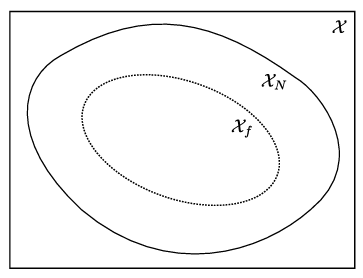
\includegraphics[width=0.6\linewidth]{figures/feasible_set.png}
    \caption{ Illustration of the constrained set \(\mathcal{X}\), the set of feasible initial conditions \( \mathcal{X_N}  \),
 and the terminal region \( \mathcal{X_f} \) \cite{maiworm2021gaussian} .}
    \label{fig:enter-label}
\end{figure}


To achieve recursive feasibility, we need to ensure that the state \( x \) remains within \( \mathcal{X_N} \) for all time steps, i.e., \( \mathcal{X_N}  \) must be control invariant for \( x^+ = f(x,u) \) with the MPC control law \( u = \kappa_{MPC}(x_k) \). The necessary assumption on this regard is the following
\begin{assumption}\label{assumption:assumption4}
    (Control Invariant Terminal Region:) The terminal region \( \mathcal{X_f} \subseteq X \) is compact, contains the origin, and is control invariant for \( x^+ = f(x,u) \), where \( u \in \mathcal{U} \).
\end{assumption}

\begin{proposition}\label{ps:proposition2}
   It states that if Assumptions \ref{assumption:assumption2} to \ref{assumption:assumption4} hold, then \( X_N \) is positive invariant for \( x_{k+1} = f(x_k, \kappa_{MPC}(x_k)) \).
\end{proposition}
For the complete proof of Proposition \ref{ps:proposition2}, refer to \cite{rawlings2009model}. The underlying idea is to begin with \( X_0 := X_f \) and define \( X_1 = \{x \in X : \exists u \in U \text{ such that } f(x,u) \in X_0\} \).

The key approach to achieving recursive feasibility is to steer the state using MPC towards the terminal region \( X_f \) and then switch to a terminal controller \( \kappa_f(x) \) that maintains \( X_f \) invariant. This terminal controller is not usually applied in practice; rather, it serves as a means to ensure recursive feasibility. 



% \subsection{ Online Learning of GP-based Transition Prediction
%  Models}\label{sec:section3.2}

 
\subsection{GP-MPC Framework }\label{sec:section3.2}
 Gaussian process regression (GPR) was introduced as a powerful technique for estimating unknown output latent functions. The posterior mean function $m^+(w|D)$ serves as the desired estimator, providing a prediction of the output given the input data $D$. This posterior mean, along with the associated variance, is utilized in the Gaussian process transition model for long-term predictions, as outlined in equation (\ref{eq:single_prediciton}). At each iteration of the algorithm, long-term predictions are computed using the Gaussian Process model trained on historical data. These predictions serve as the basis for formulating the optimal control problem\cite{kamthe2018}. The quadratic cost function is defined using these long-term predictions, capturing the trade-offs between control effort and performance objectives. Using the long-term predictions and the defined cost function, the optimal control problem is formulated. This problem incorporates state and control input constraints, ensuring that the resulting control inputs satisfy system limitations. The objective is to find control inputs that minimize the cost function while adhering to the constraints.
 
 The formulated optimal control problem is solved using a nonlinear optimizer. This optimizer searches for optimal control inputs that minimize the cost function subject to the imposed constraints. Various optimization techniques, such as gradient-based methods or evolutionary algorithms, can be employed depending on the complexity of the problem. Once the optimal control inputs are obtained, the first element of the optimal control input sequence is applied to the plant's dynamics equation. The resulting states are measured, and the data set is updated with the new measured states. This updated data set is then used to train the Gaussian Process model for the next iteration of the algorithm. The entire GP-MPC framework, represented by Algorithm \ref{alg:gp_mpc}, is repeated over the prediction horizon $N$. This iterative process allows the control system to adapt to changing dynamics and uncertainties over time, resulting in effective and robust control performance.
 
 In this section, we outline our approach for the recursive Gaussian Process-Model Predictive Control (GP-MPC) framework. In the recursive GP-MPC framework, firstly GP model learning, where we learn a prediction model only from measured input-output data using a Gaussian process, as explained in the section \ref{sec:section2.1}. Next, Controller design, where we design a Model Predictive Controller to tackle the control problem using the posterior distribution from the GP-trained model for long-term prediction. Additionally, we employ a nonlinear optimizer to solve the optimal control problem effectively.



\begin{algorithm}
    \caption{Gaussian Process Model Predictive Control}
    \label{alg:gp_mpc}
    \textbf{Initialization:}
    \begin{enumerate}
        \item \textbf{GP Parameters:} Prior mean \( m(\cdot) \), covariance function \( K(\cdot,\cdot) \), likelihood function, inference function, initial hyperparameters \( \theta \).
        \item \textbf{MPC Parameters:} Prediction horizon \( N \), initial conditions, input constraints, state constraints, hard input constraint set \( \mathcal{U} \), state constraint set \( \mathcal{Y} \), Weighting matrices \( Q \) and \( R \).
        \item \textbf{Data Set:} Initialization required Data set \( \mathcal{D} \).
    \end{enumerate}
    \textbf{Recursion:} \textbf{for }{$i \gets 1$ to $N$} \textbf{ do}
    \begin{algorithmic}[1]
        \State Initialization: initial input \( u_0 \) = first element \( u_k = \kappa_{\text{MPC}}(\mathbf{x}_k | \mathcal{D}_k) = \hat{u}_{k|k}^* \).
        \State \textbf{Training the GP model:} Repeat - \textbf{for} each state \( x \) \textbf{do}
        \begin{itemize} 
            \item Optimize hyper parameters \( \theta \) with initial data set \(\mathcal{D}\).
            \item Compute GP Posterior Eq. (\ref{eq: NL_pd_implicit}).
            \item Predict mean \( m(\cdot) \), covariance matrix \( \Sigma(\cdot,\cdot) \) at time step \(k+1\) using Posterior GP.
        \end{itemize}
        \State \textbf{Model Predictive Controller Design}
        \begin{itemize}
            \item Compute long-term prediction over the control horizon.
            \item Compute cost function see Section \ref{sec:costfunc}.
            \item Formulate Optimal Control Problem see Section \ref{sec:ocp}.
            \item Solve OCP for initial conditions : state \(x_k\), input \( u_0 \). 
        \end{itemize}
        \State \textbf{Update}
        \begin{itemize}
            \item Apply first element optimal control input \(u_k=\kappa_{\mathrm{MPC}}\left(\boldsymbol{x}_k \mid \mathcal{D}_k\right)=\hat{u}_{k \mid k}^*\) to plant.
            \item Obtain new output \(x_{k+1}\).
            \item Construct new GP data point \(\left(\boldsymbol{\tilde{x_k}}, x_{k+1}\right) \) with \(\boldsymbol{w}_k=\left(\boldsymbol{\tilde{x}}_k, u_k\right)\) to Data Set \(\mathcal{D}\).
            \item repeat.
        \end{itemize}
    \end{algorithmic}
\end{algorithm}



\begin{algorithm}
\caption{Training the Gaussian Process model}
\label{alg:gp_model}
\renewcommand{\algorithmicrequire}{\textbf{Input:}}
\renewcommand{\algorithmicensure}{\textbf{Output:}}
    \begin{algorithmic}
    \Require {$X_k$, $U_k$, $X_{k+1}$ Observation data \\ 
             \quad   $n_x,n_u$ number of state variables, inputs \\
            \quad $cov \gets \{@covSEard\}$ \\
            \quad $mean \gets \{@meanLinear\}$ \\
            \quad $lik \gets \{@likGauss\}$ \\
            \quad $inf \gets \{@infGaussLik\}$ \\
            \quad $hyp_0$ initial hyperparameters } \\
            \quad number of conjugate gradient steps $N_{\text{cg}} = 100$
    \Ensure {$x_{k+1}(\mu,\sum) $}
    \end{algorithmic}

    \begin{algorithmic}[1]
    \For{$i \gets 1$ to $n_x$}
        \If{$N_{\text{cg}} == 0$}
            \State $hyp \gets hyp0$
        \Else
            \State $hyp.\text{state}(i) \gets \text{fitGP}(\text{state}(i).hyp0,..)$ \quad \text{//hyperparameter optimization}
            % (hyp_1, \text{inf}, \text{mean}, \text{cov}, \text{lik}, x_{\text{trc}}, y_{\text{tr}}(:,i), [])$
        \EndIf
        \State $x_{k+1}(i)[\mu,\sum] \gets \text{gp}(\text{state}(i).hyp,...)$ \text{// prediction of $x_{k+1}$ for each state }
        
        % \text{inf}, \text{mean}, \text{cov}, \text{lik}, x_{\text{trc}}, y_{\text{tr}}(:,i), x_{\text{trc}}(end,:))$
    \EndFor
    
    \State \textbf{return} $x_{k+1}(\mu,\sum)$

\end{algorithmic}
\end{algorithm}






\subsubsection{GP Model Learning}
In the recursive GP-MPC framework, the first step is GP model learning. Here, we aim to learn a prediction model solely from measured input-output data using a Gaussian process, as explained in Section \ref{sec:section2.1}. The Gaussian process regression is a powerful technique for estimating unknown output latent functions. Gaussian process regression allows us to model complex relationships between inputs and outputs without assuming a specific parametric form for the underlying function. This flexibility makes GP particularly suitable for modeling systems with nonlinear dynamics or uncertain behavior. 

During GP model learning, we utilize the available input-output data to train the Gaussian process model. This involves estimating the hyperparameters of the kernel function and learning the posterior distribution over functions. The learned model provides predictions of the output given new input data, along with uncertainty estimates, which are crucial for robust control design. The posterior mean function $m^+(w|D)$ serves as the desired estimator, providing a prediction in the form of a gausiian distribution in terms of mean and variance. This posterior mean, along with the associated variance, is utilized in the Gaussian process (GP) transition model for long-term predictions, as outlined in equation (\ref{eq:single_prediciton}).

To adapt to changing processes and environments, an online learning approach for the Gaussian process is introduced. This approach updates the training dataset during operation and optimizes the hyperparameters according to the dataset used to compute the posterior distribution. This ensures that the model remains accurate and effective in capturing the underlying dynamics of the system, even as they evolve over time.


Selecting appropriate hyperparameters is crucial for ensuring accurate predictions. The normal algorithm successfully identifies the minimum of the target function, demonstrating its efficacy in optimization tasks. However, it becomes evident that improper hyperparameter selection can hinder convergence, undermining the required assumptions for safe exploration. Interestingly, even with larger initial length scales, convergence is attainable across different starting points, provided the non-constant segments are adequately evaluated. Subsequently, during initial optimization, these length scales are reduced, gradually fine-tuning with an increasing number of data points to better approximate the target function.

Employing gradient-based optimizers alongside larger length scales and elevated noise standard deviation ($\sigma_n$) poses a risk: the maximum likelihood estimate may falter, converging to a local minimum instead of the desired global minimum, as depicted. This scenario necessitates careful consideration and the adoption of strategies outlined in Section \ref{sec:optimize_hy} to mitigate such challenges. The \texttt{fitGP} function is employed for this purpose, which optimizes the hyperparameters using the gradient descent method. The literature (\cite{LUBSEN20233079}) extensively discusses approaches to address converging to a local minimum issue, emphasizing the importance of tailored methodologies for robust optimization. These strategies encompass various techniques aimed at enhancing algorithmic resilience and fostering convergence towards global minima, thereby bolstering the reliability and efficacy of optimization processes.

In summary, the report discusses the utilization of Gaussian process regression for long-term prediction, introducing an online learning approach for adaptation to changing environments. The \texttt{fitGP} function is highlighted as a tool for efficiently optimizing hyperparameters, ensuring accurate predictions even as the system dynamics evolve.

In summary, the algorithm of Gaussian Process model is shown in detail in Algorithm \ref{alg:gp_model} training the report delves into the application of Gaussian process regression (GP) for long-term prediction, offering insights into its effectiveness in capturing complex relationships between inputs and outputs without relying on specific parametric forms. The introduction of an online learning approach enhances the adaptability of GP models to evolving environments, allowing for continuous updates and refinement based on incoming data.

Furthermore, robust optimization strategies play a crucial role in model training, especially in mitigating the risk of converging to local minima during the optimization process. By carefully selecting hyperparameters and employing gradient-based optimizers alongside larger length scales and elevated noise standard deviation, the algorithm can navigate complex optimization landscapes more effectively, ultimately improving the overall performance and efficacy of the predictive modeling framework. To ensure the reliability and adaptability of long-term prediction models in dynamic environments with uncertainty, the better performance and efficacy of the GP model are crucial, which highlighting the importance of adaptive learning approaches and efficient hyperparameter optimization techniques.

\begin{algorithm}
\caption{Function: long-term prediction }
\label{alg:long_term_prediction}
\renewcommand{\algorithmicrequire}{\textbf{Input:}}
\renewcommand{\algorithmicensure}{\textbf{Output:}}
    \begin{algorithmic}
    \Require {augmented data matrix $\tilde{X_k} =[X_k, U_k]$, \\ 
    \quad \quad \quad one-step ahead state data $Y = X_{k+1}$, \\
    % \quad Posterior Prediction $x_{k+1}[\mu,\sum] $, \\
    \quad \quad \quad $\text{augmented mean matrix } \tilde{\boldsymbol{\mu}}_{k+1} = \begin{bmatrix} \mu_{x_{k+1}} , u^* \end{bmatrix}$, \\
    \quad \quad \quad $\text{augmented covariance matrix } \tilde{\boldsymbol{\sum}}_{k+1} = \begin{bmatrix} \Sigma_{x_{k+1}} & 0 \end{bmatrix}$, \\
    \quad \quad \quad GP hyperparameters {$\Lambda, \sigma_{w}, \sigma_{f}$}, \\ \quad \quad \quad $n_x,n_u$ number of state variables, inputs}
    \Ensure {$x(\mu^*,\sum^*) $}
    \end{algorithmic}
\begin{algorithmic}[1]
    \For{$k = 1$ to $n_x$}
        \For{$i = 1$ to $n_x$}
            \State $\boldsymbol{\beta}_i \gets \left(\boldsymbol{K}_i+\sigma_{w_i}^2\right)^{-1} {Y_i} $ 
            \State $\nu \gets \left(\tilde{\boldsymbol{x}}-\tilde{\boldsymbol{\mu}}_{k+1}\right)$
            \State Compute $q_i$ \qquad \qquad // equation (\ref{eq:mu_qa})
            \State ${R_i}  \gets \tilde{{\Sigma}}_t\left({\Lambda}_a^{-1}+{\Lambda}_b^{-1}\right)+{I}$ 
            \State ${T_i} \gets {\Lambda}_a^{-1}+{\Lambda}_b^{-1}+\tilde{{\Sigma}}_t^{-1}$
            \State ${z}_{i} \gets \Lambda_a^{-1}.*{\nu}+{\Lambda}_b^{-1}.*{\nu}$
            \State Compute $ Q_{i}$ \qquad \qquad // equation (\ref{eq:Qij})
        \EndFor
        \State Calculate $\mu_k$ \qquad \qquad // equation (\ref{eq:mu})
    \EndFor
    
    \For{$i = 1$ to $n-1$}
        \For{$j = 1$ to $n-1$}
            \If{$i==j$}
                \State Calculate $\sum(i,i)$   \qquad \qquad // equation (\ref{eq:sigma_aa})
            \Else
                \State Calculate $\sum(i,j)$ and $\sum(j,i)$ \qquad \qquad // equation (\ref{eq:sigma_ab})
            \EndIf
        \EndFor
    \EndFor

\end{algorithmic}
\end{algorithm}





\subsubsection{Controller Design}\label{sec:controllerdesign}

Following GP model learning, the next step in the recursive GP-MPC framework is Controller design. Here, we leverage the learned Gaussian process model to design a Model Predictive Controller for tackling the control problem. MPC is a control strategy that repeatedly solves an optimization problem over a finite prediction horizon, taking into account the system dynamics and constraints, to generate optimal control inputs. 

\begin{equation} \label{eq:modified_ocp}
    \begin{aligned}
 & \underset{u^*_k}{\text{minimize}} \ J(k) = \sum_{k=i}^{i+N-1}( x_k^T Q x_k + u_k^T R u_k )  \\
 \text{subject to}\\
& x_{k+1} = f(x_k, u_k) + \epsilon \quad \text{for } k=i \\
& u_{\text{min}} \leq u_k \leq u_{\text{max}} \quad \text{for } k=i,\ldots,i+N-1 \\
& A x_k \leq B \quad \text{for } k=i,\ldots,i+N-1 \\
\end{aligned}
\end{equation}

This enables us to incorporate uncertainty into the control decision-making process, leading to more robust and adaptive control strategies. The formulation of the optimal control problem holds significant importance in the design of a controller. At its core, the optimal control problem aims to determine the best sequence of control inputs over time to optimize a certain objective while adhering to system dynamics and constraints. This problem formulation is crucial for designing efficient and robust control strategies in complex systems where achieving desired performance while considering limitations and uncertainties is paramount. As discussed in Section \ref{sec:ocp}, we need to ensure the feasibility and stability of the optimal control problem. The modified Model Predictive Control optimal control problem can be seen in Equation \eqref{eq:modified_ocp}. We aim to make states zero with minimal control input, i.e., our set point is zero. If we want to track the reference signal or change the set point to another value, then we need to modify Equation (\ref{eq:modified_ocp}) with $(x_k - x_{\text{ref}})$. The simple state and control input constraints are subjected to an optimal control problem (OCP). To solve the OCP, it requires state prediction over the prediction horizon from $k = i, \ldots, i + N - 1$, these predictions should be accurate and efficient in defining the actual dynamics of the plant model with uncertainty. 

In our framework, we use the posterior distribution obtained from the Gaussian Process -trained model for long-term prediction within the Model Predictive Control  formulation. This enables us to incorporate uncertainty into the control decision-making process, leading to more robust and adaptive control strategies. For this, we introduce moment-matching approximation as a long-term prediction model which provides more accurate and efficient predictions considering uncertainty into account. The concept is very simple: predicting the control inputs using GP hyperparameters and posterior prediction, as outlined in Algorithm \ref{alg:long_term_prediction}.

A key aspect of the GP-MPC formulation is the utilization of the predicted mean and variance from the GP model for online predictions. The moment-matching approximation facilitates efficient computation of these quantities, enabling real-time decision-making in control applications. All the predictions from moment-matching approximation are Gaussian distributed in terms of mean and variance. By focusing on the mean prediction and omitting the consideration of variance dynamics for simplicity, the GP-MPC framework strikes a balance between computational complexity and predictive accuracy.

In the Gaussian Process Model Predictive Control (GP-MPC) framework, leveraging Gaussian process regression for long-term prediction introduces a flexible and probabilistic approach to modeling system dynamics. By incorporating the GP model alongside the nominal model $f(x_k, u_k)$, the GP-MPC problem formulation extends beyond traditional deterministic models, offering enhanced adaptability to uncertain or nonlinear system behaviors.

Furthermore, constraint handling in the GP-MPC formulation is crucial for ensuring the feasibility and stability of the control solutions. Finally, a nonlinear optimal control problem is formulated, which can be solved to find optimal control inputs. Additionally, to solve the optimal control problem effectively, we employ a nonlinear optimizer, which efficiently handles the nonlinearities and constraints inherent in many real-world control problems. The nonlinear optimizer that we used is \texttt{fmincon}, and there are other nonlinear optimizers \cite{verschueren2019acados}. The solution, which is optimal control inputs, satisfies specified bounds while optimizing performance objectives, thereby enhancing the robustness and safety of the control system. Finally, the MPC controller is designed and formulated as outlined in Algorithm \ref{alg:mpc}. 

Overall, the integration of Gaussian process regression into model predictive control offers a promising avenue for addressing challenges associated with uncertain and nonlinear system dynamics. By leveraging probabilistic modeling techniques and advanced optimization methods, GP-MPC facilitates robust and adaptive control strategies capable of handling real-world complexities and uncertainties. Continued research in this area holds the potential to further advance the capabilities and applicability of GP-MPC in diverse engineering and autonomous systems domains.

\begin{algorithm}
\caption{MPC controller }
\label{alg:mpc}
\renewcommand{\algorithmicrequire}{\textbf{Input:}}
\renewcommand{\algorithmicensure}{\textbf{Output:}}
    \begin{algorithmic}
    \Require {$u_0$ initial control inputs \\
        \qquad \quad $X_k$, $U_k$, $X_{k+1}$ observation data \\
        \qquad \quad $\mu_{x_{k+1}}, \Sigma_{x_{k+1}}$ posterior GP prediction \\
        \qquad \quad $Q$: Array of weightings for the state variables \\
        \qquad \quad $R$: Weighting for the control inputs \\
        \qquad \quad GP hyperparameters \\
        \qquad \quad $A, B$ state constraints matrices \\
        \qquad \quad $U_a, U_b$ control input constraints 
        }
    \Ensure {$u^*$ optimal control inputs}
    \end{algorithmic}
    
    \begin{algorithmic}
    \State $fun \gets @(u0) \quad COST(...) $  \qquad \qquad cost function 
    \State $u^* \gets fmincon(fun)$ \qquad \qquad // Nonlinear optimization  \\ 
    \end{algorithmic}


\begin{algorithmic}[1]
\Function{cost}{$u_0, \tilde{X}, \mu, \Sigma, hyp, X_{k+1}, Q, R$}
    \State Prediction horizon $N$
    \State $J \gets 0$
    \For{$i = 1$ to $N$}
        \If{$i == 1$}
            \State $\tilde{\mu} \gets [\mu_{k-1}, u_0(i)]$
            \State $\tilde{\Sigma} \gets \text{blkdiag}(\Sigma, 0)$
        \Else
            \State $\mu \gets [\mu^*(i-1), u_0(i)]$
            \State $\tilde{\Sigma} \gets \text{blkdiag}(\Sigma^*(i-1), 0)$
        \EndIf
    \State $[\mu^*(i), \sum^*(i)] \gets $ long term prediction function \qquad \qquad //algorithm \ref{alg:long_term_prediction}
            \State $J \gets J + \mu^*(i) \cdot Q \cdot \mu^*(i) + u_0(i) \cdot R \cdot u_0(i)$ \qquad \qquad // equation  (\ref{eq:cost_function})
    \EndFor
    \State \textbf{return} $J$
\EndFunction
\end{algorithmic}

\end{algorithm}


% \subsection{Hardware}

% Room N1059 is a computer pool for students to work in. You can use MATLAB/SIMULINK 
% there to do your calculations and write your thesis.


% \subsection{Software}

% There are different editors for \LaTeX. Some frequently used at the institute are TeXnicCenter and Texmaker. 
% If you use TeXnicCenter you can import the file \linebreak \verb"Ausgabeprofile\_TeXnicCenter.tcp", in that folder, by 
% \textit{Ausgabe - Ausgabeprofile definieren... - Importieren}. Choose the output-profile \verb!\LaTeX => PS => PDF student-thesis!. 
% Thus the settings should be correct and a PDF of your work should be generated. If that does not work, check the settings for proper
% paths to the post-processing and viewer programs.

% Visio as graphical software is provided. If you produce figures directly with MATLAB, consider the export-setting of the ''print'' command.

% \subsection{References}

% The institute uses a common literature database, where a lot of books and articles that you may want to cite are already included. 
% The respective \texttt{bib}-file can be found on \verb"S:\ICS library\ics.bib".
% Copy the most recent version to your root directory of your thesis!

% Then, you can open this file with your \LaTeX\ editor or you can use a literature manager like ''jabref'', for instance.
% Check if the reference that you want to cite is included. In this case, you can simply use the BiB\TeX-key in the respective command.
% The literature information is properly generated only, if \texttt{bibtex} is be executed twice: first \verb!bibtex pd! and then \verb!bibtex main!. 
% If you use TeXnicCenter and the provided output-setting, this is done automatically. In other cases, the easiest way would be to use
% the \texttt{build.cmd} file that accompanies this template. It will execute the compilation process in the proper order and open the pdf file
% afterwards.

% Please provide with your thesis complete information on your references (title, authors, date, DOI, maybe even pdf files). We would like to
% include these in our database, if this has not already happened..


% \subsection{Binding the work}

% The institute offers you to print and bind the work. You need three copies in general, one for your supervisor, one for the Professor and one for yourself, and maybe more. 
% After finalizing your work, it is also included in the literature database by your supervisor.

% Your work is printed in the correct order. Put a transparent film in the front and a cardboard in the back.

% Your work is stapled. Look for staples of the right length in the shelf in the computer pool and use the
% large stapler. Afterwards tape the back of your work. You will find illustrative material in the bibliography.

% In addition to your printed work, you have to hand in a cd with the pdf file of your work and other important files. 
% Please structure them well, such that some years later somebody else is able to find the important things. The CD 
% is fixed inside your work at the back within a paper cover.

% Last but not least, do not forget to sign the declaration.